\begin{figure*}
  \begin{subfigure}[b]{0.5\textwidth}
    \begin{tikzpicture}
      \datavisualization [
        scientific axes=clean,
        x axis={label={$N$}},
        y axis={label={Predicted}},
        visualize as line/.list={fit, pred},
        fit={style={color=red}},
        pred={style={color=blue}},
      ]
      data[headline={x, y}, read from file=tests/data/fit_known_4.csv,
        set=fit]
      data[headline={x, y}, read from file=tests/data/pred_known_4.csv,
        set=pred]
      ;
    \end{tikzpicture}
  \end{subfigure}
  \begin{subfigure}[b]{0.5\textwidth}
    \begin{tikzpicture}
      \datavisualization [
        scientific axes=clean,
        x axis={label={$N$}},
        y axis={label={Accuracy}},
        visualize as line/.list={fit, pred},
        fit={style={color=red}},
        pred={style={color=blue}},
      ]
      data[headline={x, y}, read from file=tests/data/fit_acc_4.csv,
        set=fit]
      data[headline={x, y}, read from file=tests/data/pred_acc_4.csv,
        set=pred]
      ;
    \end{tikzpicture}
  \end{subfigure}
  \begin{flushright}
    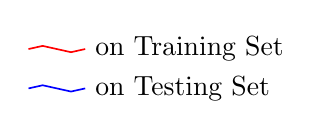
\begin{tikzpicture}
      \draw[red,semithick] (0,.5) -- (.18,.54) --
        (.54,.46) -- (.72,.5) node[right,black]
        {on Training Set};
      \draw[blue,semithick] (0,0) -- (.18,.04) --
        (.54,-.04) -- (.72,0) node[right,black]
        {on Testing Set};
    \end{tikzpicture}
  \end{flushright}
\end{figure*}

